\documentclass[12pt,a4paper]{article}
\usepackage{cmap} % Makes the PDF copiable. See http://tex.stackexchange.com/a/64198/25761
\usepackage[T1]{fontenc}
\usepackage[brazil]{babel}
\usepackage[utf8]{inputenc}
\usepackage{amsmath}
\usepackage{amsfonts}
\usepackage{amssymb}
\usepackage{amsthm}
\usepackage{textcomp} % \degree
\usepackage{gensymb} % \degree
\usepackage[usenames,svgnames,dvipsnames]{xcolor}
\usepackage{hyperref}
\usepackage{multicol}
\usepackage{graphicx}
\usepackage[margin=2cm]{geometry}

\hypersetup{
    colorlinks = true,
    allcolors = {blue}
}

\newcommand{\fixme}{{\color{red}(...)}}

\newcommand*\sen{\operatorname{sen}}
\newcommand*\senh{\operatorname{senh}}
\newcommand*\abs[1]{\left|#1\right|}
\newcommand*\dom[1]{\operatorname{Dom}\left(#1\right)}

\newcommand*\R{\mathbb{R}}

\newcommand*\tipo{PROVA III}
\newcommand*\turma{ELE141-01U}
\newcommand*\disciplina{CDI0001}
\newcommand*\eu{Helder G. G. de Lima}
\newcommand*\data{18/11/2015}

\author{\eu}
\title{\tipo - \disciplina}
\date{\data}

\begin{document}
\thispagestyle{empty}
\newgeometry{margin=2cm,bottom=0.5cm}
\begin{center}

\includegraphics[width=9.0cm]{marca}
\noindent\begin{tabular}{l c c r}
  \textbf{\disciplina (\turma)}
& \textbf{\tipo}
& \textbf{\data}
\end{tabular}
\\ Prof. \eu\footnote{
Este é um material de acesso livre distribuído sob os termos da licença \href{https://creativecommons.org/licenses/by-sa/4.0/deed.pt_BR}{Creative Commons BY-SA 4.0}.}
\end{center}

\noindent Nome do(a) aluno(a): \rule{13cm}{0.01cm}

%\section*{Instruções}
\begin{center}\fbox{
\begin{minipage}{14cm}

{\footnotesize
\begin{itemize}
\renewcommand{\theenumi}{\Roman{enumi}}
\item Identifique-se em todas as folhas.
\item Mantenha o celular e os demais equipamentos eletrônicos desligados durante a prova.
\item Justifique cada resposta com cálculos ou argumentos baseados na teoria estudada.
\item Resolva (integralmente) apenas os itens de que precisar para somar 10,0 pontos.
\end{itemize}
}

\end{minipage}
}
\end{center}


%\section*{Questões}

\begin{enumerate}

\item (3,0) Calcule os seguintes limites, utilizando as regras de L'Hôpital quando for apropriado.
\begin{multicols}{3}
\begin{enumerate}
\item $\displaystyle\lim_{x\to\infty} \frac{x+\sin(x)}{x}$
\item $\displaystyle\lim_{x\to +\infty} (x+1)^{\frac{1}{\ln{x}}}$
\item \footnotesize $\displaystyle\lim_{x\to 0^+} \ln(e^2 x)\nolinebreak-\nolinebreak\ln(\sen(e x))$
\end{enumerate}
\end{multicols}

\item (1,0) Explique o erro (com um exemplo simples que mostre o problema) no seguinte raciocínio:

``Como a derivada da função $f$ no ponto $a$ é zero e a segunda derivada de $f$ em $a$ também é zero, este não é um ponto de máximo, nem um ponto de mínimo.''

\item (3,0) Esboçar $f(x) = x\abs{x} - 2\pi x$, explicitando o domínio, simetrias, zeros, intervalos de crescimento e decrescimento, pontos de máximo e mínimo, concavidade, pontos de inflexão, assíntotas e limites que forem relevantes. Não esqueça de justificar suas afirmações!

\item (1,5) Determine as equações de todas as assíntotas (horizontais, verticais e/ou oblíquas) da função $f(x) = \tanh(x) + \abs{x} + 2$, sabendo que $\tanh(x) = \dfrac{\senh(x)}{\cosh(x)} =  \dfrac{e^x - e^{-x}}{e^x + e^{-x}}$.

\item (2,0) Uma bateria de voltagem fixa $V$ e resistência interna fixa $r$ está ligada a um circuito de resistência variável $R$. Pela Lei de Ohm, a corrente no circuito é $I = \frac{V}{R+r}$. Se a potência é dada por $P = I^2R$, mostre que a potência máxima ocorre quando $R = r$.

\item (1,5) Faça um esboço do gráfico de $f$, assumindo que$f: [-4, +\infty) \to \R$ seja uma função derivável cujo gráfico passa por $A=(-4,-4)$, e cuja derivada tem o seguinte gráfico:

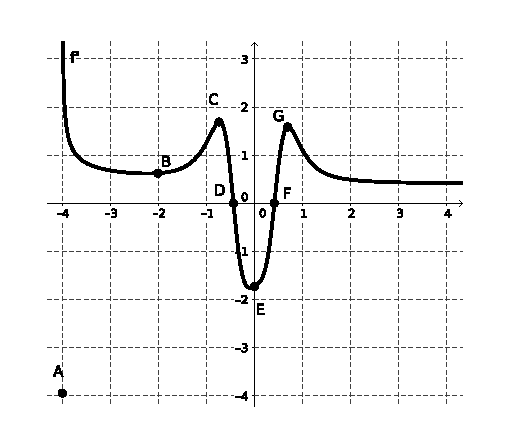
\includegraphics[width=8.7cm]{img/prova-3-ele-grafico-f'}

\end{enumerate}

\newpage
\restoregeometry
\section*{Respostas e observações}

\begin{enumerate}

\item \textit{Calcule os seguintes limites, utilizando as regras de L'Hôpital quando for apropriado.}
\begin{enumerate}
\item $\displaystyle\lim_{x\to\infty} \frac{x+\sen(x)}{x}$
\[
\lim_{x\to\infty} \frac{x+\sen(x)}{x}
= \lim_{x\to\infty} 1 + \frac{1}{x} \sen x
= 1 + 0
=  1,
\]
pois $\sen x$ é uma função limitada, e $\lim_{x\to\infty} \frac{1}{x} = 0$.

\textbf{Obs}: Não é permitido aplicar a regra de L'Hôpital neste caso, pois para que ocorresse
\[
\lim_{x\to\infty} \frac{(x+\sen(x))^\prime}{x^\prime}
= \lim_{x\to\infty} \frac{1+\cos(x)}{1}
= \lim_{x\to\infty} 1 + \cos x
\]
seria preciso que este último limite existisse. Mas $\cos(x)$ é uma função periódica tal que, para todo $k \in \mathbb{Z}$, tem-se $\cos(k \cdot 2\pi) = 1$ e $\cos( \pi + k \cdot 2\pi ) = -1$. Portanto não existe $\lim_{x\to\infty} 1 + \cos x$.

\item $\displaystyle\lim_{x\to +\infty} (x+1)^{\frac{1}{\ln{x}}}$

Seja $L = \lim_{x\to +\infty} (x+1)^{\frac{1}{\ln{x}}}$. Então:
\begin{align*}
\ln(L)
& = \ln\left( \lim_{x\to +\infty} (x+1)^{\frac{1}{\ln{x}}} \right)
  = \lim_{x\to +\infty} \ln\left( (x+1)^{\frac{1}{\ln{x}}} \right)
  = \lim_{x\to +\infty} \frac{1}{\ln{x}} \ln\left(x+1\right) \\
& = \lim_{x\to +\infty} \frac{\ln(x+1)}{\ln{x}}
  = \lim_{x\to +\infty} \frac{\frac{1}{x+1}}{\frac{1}{x}}
  = \lim_{x\to +\infty} \frac{x}{x+1}
  = \lim_{x\to +\infty} \frac{1}{1+0}
  = 1.
\end{align*}
Como $\ln(L) = 1$, conclui-se que $L = e^{\ln(L)} = e^1 = e$.
\item $\displaystyle\lim_{x\to 0^+} \ln(e^2 x)\nolinebreak-\nolinebreak\ln(\sen(e x))$
\begin{align*}
\lim_{x\to 0^+} \ln(e^2 x)-\ln(\sen(e x))
& = \lim_{x\to 0^+} \ln\left(\frac{e^2 x}{\sen(e x)}\right)
  = \ln\left( \lim_{x\to 0^+} \frac{e^2 x}{\sen(e x)}\right) \\
& = \ln\left( \lim_{x\to 0^+} \frac{e^2}{e \cos(e x)}\right)
  = \ln\left( \frac{e}{\cos(0)}\right)
  = \ln\left( e \right) = 1.
\end{align*}
\end{enumerate}

\item \textit{Explique o erro (com um exemplo simples que mostre o problema) no seguinte raciocínio:}

\textit{``Como a derivada da função $f$ no ponto $a$ é zero e a segunda derivada de $f$ em $a$ também é zero, este não é um ponto de máximo, nem um ponto de mínimo.''}

É preciso mais informações sobre a função para poder concluir que $a$ não é ponto de máximo nem de mínimo, pois o teste da segunda derivada é inconclusivo sobre os pontos críticos em que ela zera. Por exemplo:
\begin{itemize}
\item Uma função como $f(x) = x^4$, para a qual $f^\prime(x) = 4x^3$ e $f^{\prime \prime } = 12x^2$, satisfaz ambas as condições $f^\prime(0) = 0$ e $f^{\prime\prime}(0) = 0$, mas tem um ponto de mínimo em $x=0$, pois o sinal da primeira derivada é negativo para $x<0$ e positivo para $x>0$ (ou seja, $f$ é decrescente antes da origem e crescente depois dela, passando por um ponto de mínimo).
\item Caso $f$ esteja sendo considerada apenas em um intervalo fechado, que tem $a$ como um de seus extremos, ele ainda poderia ser um ponto de máximo ou de mínimo. Considere por exemplo a função $f(x) = x^3$ em qualquer intervalo $[0, b]$ (com $b \in \R^*_+$). Tem-se $f^\prime(x) = 3x^2$ e $f^{\prime \prime }(x) = 6x$, de modo que $f^\prime(0) = f^{\prime\prime}(0) = 0$. Mas $f$ é crescente em $[0,b]$, pois $f^\prime(x) > 0$ para $x \neq 0$.
\end{itemize}


\item \textit{Esboçar $f(x) = x\abs{x} - 2\pi x$, explicitando o domínio, simetrias, zeros, intervalos de crescimento e decrescimento, pontos de máximo e mínimo, concavidade, pontos de inflexão, assíntotas e limites que forem relevantes. Não esqueça de justificar suas afirmações!}

Observe inicialmente que $f(x)
= \begin{cases}
x^2-2\pi x, \text{ se } x \geq 0 \\
-x^2-2\pi x, \text{ se } x < 0
\end{cases}$
está definida em todos os números reais, isto é,
$\dom{f} = \R$. Além disso, tem-se
\[
f(-x)
= -x \abs{-x} - 2 \pi (-x)
= -( x \abs{x} - 2 \pi x )
= -f(x),\]
ou seja, $f$ é uma função ímpar (seu gráfico é simétrico em relação à origem). A função possui trez zeros, pois
\[
f(x) = 0
\Leftrightarrow x\abs{x} - 2\pi x = 0
\Leftrightarrow x(\abs{x} - 2\pi) = 0
\Leftrightarrow x = 0 \text{ ou } \abs{x} = 2\pi.
%\Leftrightarrow x \in \{-2\pi, 0, 2\pi\}.
\]

Como $f$ é contínua em $\R$, não há nenhum ponto $a \in \R$ tal que $\lim_{x\to a} f(x) = \pm \infty$, logo não existem assíntotas verticais.

Também ocorre que
\[
\lim_{x\to \pm\infty} \frac{ f(x) }{x}
= \lim_{x\to \pm\infty} \frac{ x\abs{x} - 2\pi x }{x}
= \lim_{x\to \pm\infty} \abs{x} - 2\pi
= +\infty.
\]
Logo, não existem assíntotas oblíquas nem horizontais.

Em relação às derivadas de $f$, tem-se
\begin{align*}
f^\prime(x)
& = \begin{cases}
(x^2-2\pi x)^\prime, \text{ se } x > 0 \\
(-x^2-2\pi x)^\prime, \text{ se } x < 0
\end{cases} \\
& = \begin{cases}
2x-2\pi, \text{ se } x > 0 \\
-2x-2\pi, \text{ se } x < 0
\end{cases} \\
& = 2\abs{x} - 2\pi, \text{ para } x \neq 0
\end{align*}
E se $x=0$ tem-se
\[
f^\prime(0)
= \lim_{h\to 0} \frac{ (h\abs{h} - 2\pi h) - 0 }{h}
= \lim_{h\to 0} \abs{h} - 2\pi
= - 2\pi
= 2 \abs{0} - 2\pi
\]
(ou, por L'Hôpital,
$f^\prime(0)
= \lim_{x \to 0} \frac{f(x) - f(0)}{x}
= \lim_{x \to 0} \frac{f^\prime(x)}{1}
= \lim_{x \to 0} 2\abs{x} - 2\pi = - 2\pi$).
Logo, $f^\prime(x) = 2 \abs{x} - 2\pi$ para todo $x \in \R$, inclusive no zero. Como a derivada de $f$ está definida em toda a reta (é contínua), os únicos pontos críticos de $f$ serão os zeros de $f^\prime$:
\[
f^\prime(x) = 0
\Leftrightarrow 2 \abs{x} - 2\pi = 0
\Leftrightarrow \abs{x} = \pi
\Leftrightarrow x = \pi \text{ ou } x = -\pi.
\]

Além disso,
\[
f^\prime(x) < 0
\Leftrightarrow 2 \abs{x} - 2\pi < 0
\Leftrightarrow \abs{x} < \pi
\Leftrightarrow -\pi < x < \pi.
\]
de modo que $f$ é decrescente em $(-\pi, \pi)$ e crescente em $(-\infty, -\pi) \cup (\pi, +\infty)$. Consequentemente, $f$ tem um ponto de máximo local em $x=-\pi$ e um ponto de mínimo local em $x=\pi$ (nenhum deles é global, pois $\lim_{x\to \infty} f(x) = \infty$ e $\lim_{x\to -\infty} f(x) = -\infty$).
\begin{minipage}[b]{0.67\linewidth}
A concavidade de $f$ fica determinada pelo sinal de $f^{\prime\prime}$. Tem-se
\[
f^{\prime\prime}(x)
= 2\frac{\abs{x}}{x}
= \begin{cases}
2, & \text{ se } x > 0\\
-2 & \text{ se } x < 0
\end{cases}
\]
Portanto, $f$ tem concavidade para baixo em $(-\infty, 0)$ e para cima em $(0, +\infty)$, o que significa que há um ponto de inflexão em $x=0$.

\end{minipage}
\begin{minipage}[t]{0.32\linewidth}
\includegraphics[width=5.0cm]{img/prova-3-ele-3-esboco}
\end{minipage}


\item \textit{Determine as equações de todas as assíntotas (horizontais, verticais e/ou oblíquas) da função $f(x) = \tanh(x) + \abs{x} + 2$, sabendo que $\tanh(x) = \dfrac{\senh(x)}{\cosh(x)} =  \dfrac{e^x - e^{-x}}{e^x + e^{-x}}$.}

Como $f$ é uma soma/composição de funções contínuas em $\R$, ela também é contínua em $\R$, e não há nenhum ponto $p \in \R$ tal que $\lim_{x\to p} f(x) = \pm \infty$. Logo não existem assíntotas verticais. Por outro lado, tem-se
\begin{align*}
\lim_{x\to+\infty} \tanh(x)
& = \lim_{x\to+\infty} \dfrac{e^x - e^{-x}}{e^x + e^{-x}}
  = \lim_{x\to+\infty} \frac{e^x - \dfrac{1}{e^x}}{e^x + \dfrac{1}{e^x} }
  = \lim_{u\to+\infty} \frac{u - \dfrac{1}{u}}{u + \dfrac{1}{u} } \\
& = \lim_{u\to+\infty} \frac{1 + \dfrac{1}{u^2}}{1 - \dfrac{1}{u^2} }
  = \frac{1 + 0}{1 - 0 }
  = 1.
\end{align*}
Por simetria (já que $\tanh$ é ímpar), tem-se
\begin{align*}
\lim_{x\to-\infty} \tanh(x)
& = \lim_{u\to+\infty} \tanh(-u)
  = \lim_{u\to+\infty} -\tanh(u)
  = -\lim_{u\to+\infty} \tanh(u)
  = -1.
\end{align*}

Consequentemente, se $y=ax+b$ é uma assíntota em $+\infty$, então
\begin{align*}
a = \lim_{x\to+\infty} \frac{ f(x) }{x}
& = \lim_{x\to+\infty} \frac{ \tanh(x) + \abs{x} + 2 }{x}
  = \lim_{x\to+\infty} \frac{ \tanh(x) + 2 }{x} + \lim_{x\to+\infty} \frac{ \abs{x} }{x} \\
& = 0 + \lim_{x\to+\infty} \frac{x}{x}
  = 1
\end{align*}
e além disso,
\begin{align*}
b = \lim_{x\to+\infty} f(x) - ax
& = \lim_{x\to+\infty} \left( \tanh(x) + \abs{x} + 2 \right) - x
  = \lim_{x\to+\infty} \tanh(x) + x + 2 - x \\
& = \lim_{x\to+\infty} \tanh(x) + 2
  = 1 + 2
  = 3
\end{align*}
Logo, $y=x+3$ é a equação da assíntota oblíqua em $+\infty$. A assíntota $y=a_1x+b_1$ em $-\infty$ é obtida de forma análoga:
\begin{align*}
a_1 = \lim_{x\to-\infty} \frac{ f(x) }{x}
& = \lim_{x\to-\infty} \frac{ \tanh(x) + \abs{x} + 2 }{x}
  = \lim_{x\to-\infty} \frac{ \tanh(x) + 2 }{x} + \lim_{x\to+\infty} \frac{ \abs{x} }{x} \\
& = 0 + \lim_{x\to-\infty} \frac{-x}{x}
  = -1
\end{align*}
\[
b_1 = \lim_{x\to-\infty} f(x) - a_1x = \lim_{x\to-\infty} \tanh(x) + (-x) + 2 - (-x) = \lim_{x\to-\infty} \tanh(x) + 2
  = -1 + 2
  = 1
\]
Logo, $y=-x+1$ é a assíntota de $f$ em $-\infty$.

\item \textit{Uma bateria de voltagem fixa $V$ e resistência interna fixa $r$ está ligada a um circuito de resitência variável $R$. Pela Lei de Ohm, a corrente no circuito é $I = \frac{V}{R+r}$. Se a potência é dada por $P = I^2R$, mostre que a potência máxima ocorre quando $R = r$.}

No contexto deste problema pode-se assumir que $V>0$, $R>0$ e $r>0$.

\textbf{Solução 1}:
A potência é dada em função da resistência por $P = P(R) = \left( \frac{V}{R+r}\right)^2 R = V^2 \frac{R}{(R+r)^2}$. Para encontrar a potência máxima, basta encontrar um ponto crítico de $P$, tal que $P$ seja crescente antes deste ponto, e decrescente depois dele. Tem-se
\[
P^\prime(R)
= V^2 \left( \frac{R}{(R+r)^2} \right)^\prime
= V^2 \frac{(R+r)^2 - 2 R (R+r)}{(R+r)^4}
= V^2 \frac{(R+r) - 2R}{(R+r)^3}
= V^2 \frac{r - R}{(R+r)^3}
\]
Assim, $P^\prime(R) = 0 \Leftrightarrow \frac{V^2}{(R+r)^3} (r - R) = 0 \Leftrightarrow r-R=0$, e conclui-se que $R=r$ é o único ponto crítico de $P$. É claro que se $R > r$, tem-se $r-R < 0$ e $P^\prime(R) < 0$. Isso significa que $P$ é decrescente em $(r, +\infty)$. Analogamente, se $R < r$, tem-se $r-R > 0$ e $P^\prime(R) > 0$, ou seja, $P$ é crescente em $(-\infty, r)$. Portanto, $R = r$ maximiza a potência do circuito.


\textbf{Solução 2}: Como $I = \frac{V}{R+r}$, resulta que $R = \frac{V}{I}-r$. Então a potência é dada em função da corrente por $P = P(I) = I^2 R = I^2 \left( \frac{V}{I} - r \right) = IV-I^2 R$. Para encontrar a potência máxima, basta encontrar um ponto crítico de $P$, tal que $P$ seja crescente antes deste ponto, e decrescente depois dele. Tem-se
\[
P^\prime(I)
= V- 2IR
\]
Assim, $P^\prime(I) = 0 \Leftrightarrow V-2IR = 0 \Leftrightarrow V = 2IR$, e conclui-se que $I=\frac{V}{2R}$ é o único ponto crítico de $P$, e como $P^{\prime\prime}(I) = -2R < 0$, ele é um ponto de máximo. Neste caso,
\[
R
= \frac{V}{I}-r
= V\cdot \frac{2R}{V} -r
= 2R -r,
\]
ou seja, $R+r = 2R$, e consequentemente a potência do circuito é maximizada quando $R = r$.
\newpage
\item \textit{Faça um esboço do gráfico de $f$, assumindo que $f: [-4, +\infty) \to \R$ seja uma função derivável cujo gráfico passa pelo ponto $A$, e cuja derivada tem o seguinte gráfico:}

\begin{minipage}[]{0.57\linewidth}
O gráfico de $f^\prime$ indica que:
\begin{itemize}
\item $f$ é crescente de $A$ até $D$, e de $F$ em diante, pois $f^\prime$ é positiva nestes intervalos
\item $f$ é decrescente de $D$ até $F$, pois $f^\prime$ é negativa neste intervalo
\item $f$ tem concavidade para baixo de $A$ até $B$, de $C$ até $E$ e de $G$ em diante, pois $f^\prime$ é decrescente nestes intervalos
\item $f$ tem concavidade para cima de $B$ até $C$ e de $E$ até $G$, já que $f^\prime$ é crescente nestes intervalos.
\item $B$, $C$, $E$ e $G$ são pontos de inflexão, devido às mudanças de concavidade nestes pontos
\item $D$ é um ponto de máximo local de $f$, devido à mudança de crescente para decrescente neste ponto
\item $F$ um ponto de mínimo local de $f$, devido à mudança de decrescente para crescente neste ponto
\end{itemize}
\end{minipage}
\begin{minipage}[]{0.42\linewidth}
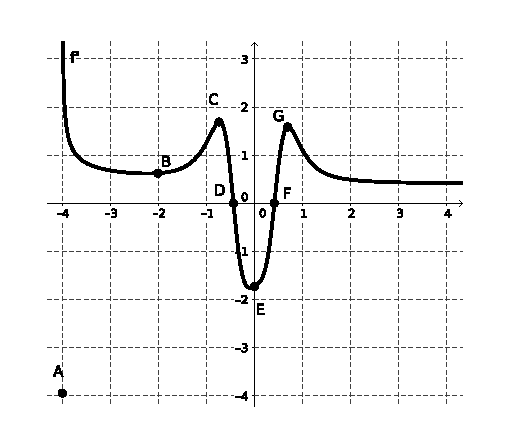
\includegraphics[width=7.4cm]{img/prova-3-ele-grafico-f'}
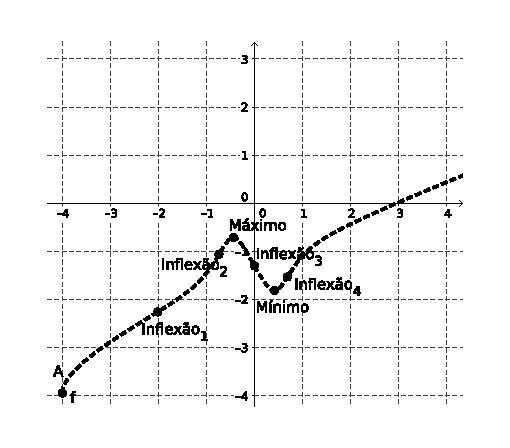
\includegraphics[width=7.4cm]{img/prova-3-ele-grafico-f}
\end{minipage}
\end{enumerate}

\end{document}
